% Cover letter using letter.sty

\documentclass[11pt]{letter} % Uses 10pt
\usepackage{graphicx,subfigure}
\usepackage{float}
\usepackage{caption}
\captionsetup{labelsep=space}

\renewcommand*{\figureformat}{\figurename~\thefigure}

\restylefloat{figure}
%Use \documentstyle[newcent]{letter} for New Century Schoolbook postscript font
% the following commands control the margins:
\topmargin=-1.2in    % Make letterhead start about 1 inch from top of page 
\textheight=14in  % text height can be bigger for a longer letter
\oddsidemargin=0pt % leftmargin is 1 inch
\textwidth=6.5in   % textwidth of 6.5in leaves 1 inch for right margin
\textheight 255mm


\begin{document}\pagenumbering{gobble}




\begin{flushleft}
{\large\bf Eamon O'Gorman}
\end{flushleft}
\medskip\hrule height 1pt
\begin{flushright}


\end{flushright} 
%\vfill % forces letterhead to top of page
{\Large 
\begin{center}
Research Accomplishments
\end{center}
}

My main research achievements to date have been associated with gaining a broader understanding into the dynamics and thermodynamics of the atmospheres of red giants (non-AGB red giants) and red supergiants (RSGs), through radio interferometric techniques. The mass-loss from these stars plays a crucial role in galactic evolution and ultimately provides much of the material required for the next generation of stars and planets. Also, a substantial fraction of the star's initial mass can be dispersed to the interstellar medium during these post main sequence evolutionary stages and this mass-loss is therefore a crucial factor governing stellar evolution, and also in explaining the frequency of supernovae in the galaxy. Despite the importance of this phenomenon, and decades of study, the specific mechanisms that drive winds from evolved spectral-type K through mid-M stars remain unknown. There is insufficient atomic, molecular, or dust opacity to drive a radiation-driven outflow and acoustic/pulsation models cannot drive the observed mass-loss rates. UV and optical observations reveal an absence of significant hot wind plasma, and the winds are thus too cool to be Parker-type thermally-driven flows. Magnetic fields are most likely involved in the mass-loss process, although current magnetic models are also unable to explain spectral diagnostics. Traditionally, observations have provided only limited disk-averaged information about the outflow environments of these stars, making it difficult to infer the wind properties. My primary research to date has focused on using the latest suite of millimeter and centimeter interferometers to provide essential spatial information on these outflow environments, to gain a better understanding of the entire mass-loss process.

Betelgeuse is one of the few nearby RSGs that can be studied in great detail across most of the electromagnetic spectrum. The extended atmosphere of this oxygen-rich RSG provides an ideal testbed for studying the poorly understood processes that drive mass-loss from K and M supergiants. Part of my research to date has focused on explaining and reconciling the puzzling results from previous single dish millimeter observations of this star's circumstellar environment. Ro-vibrational absorption lines of $^{12}$C$^{16}$O and $^{13}$C$^{16}$O by Bernat et al. (1979) revealed that Betelgeuse has undergone at least two distinct phases of mass-loss in its recent past. However, previous millimeter observations were only able to detect one component of the outflow, while the spatial extent of both components were unknown. Using multiple array configurations of the CARMA interferometer, we successfully imaged the CO($J = 2 - 1$) emission line at sub-arcsecond resolution, and for the first time were able to find the spatial extent of both outflow components, allowing their ages to be calculated (O'Gorman et al., 2012, \textit{AJ}). We also found both components to be inhomogeneous, far from the existing spherically symmetric models of its circumstellar environment, indicating a chaotic mass-loss loss process. These millimeter line emission data were obtained with the CARMA heterogeneous interferometer at Ceder Flat, California, in three different array configurations. The raw data were flagged, calibrated, and imaged using CASA. The analysis required knowledge of interferometric spatial scales and imaging techniques such as CLEAN and multi-scale CLEAN. 

The wind acceleration region is where most of the momentum and heat which drive the mass-loss in RSGs is deposited. Thermal millimeter and centimeter continuum emission directly sample this region which extends out to only a few $R_{\star}$. Spatially resolved VLA cm-continuum radio maps (Lim et al. 1998) revealed that Betelgeuse's extended atmosphere ($2-7\,R_{\star}$) was significantly cooler and much less ionized than predicted by magnetic wave models. I have been heavily involved in a collaboration which has used e-MERLIN to image the thermal continuum emission from this inner region of Betelgeuse's atmosphere at 6\,cm (Richards et al., 2013). We have discovered two chromospheric ``hotspots'' (Figure 1, \textit{left}) separated by $4\,R_{\star}$, hidden just beyond the spatial resolution of the VLA at 6\,cm. Using the astrometric solution of Harper et al. (2008), the brighter hotspot ($T_{e} > 5400$\,K) is $\sim 3.5\,R_{\star}$ from the photosphere. Inspired by this new discovery, I have analyzed multi-wavelength, multi-epoch, centimeter \textit{old} VLA data which contains the Pie Town VLBA antenna, to look for signatures of these hotspots. At the highest available frequencies, these data have even superior spatial resolution than e-MERLIN (at 6\,cm).  In Figure 1 (right) a preliminary map at 0.7\,cm is presented, and evidence of at least two features separated by only $2\,R_{\star}$ is shown. These features may be generated by  giant photospheric convective cells, although it is unlikely that such features could be accountable for the ``hotspots'' seen with e-MERLIN (O'Gorman, 2013, \textit{Thesis}).

We have recently used the Jansky Very Large Array to observe two non-dusty, non-pulsating, K spectral-type red giants at multiple radio wavelengths ($0.7 - 20$\,cm) (O'Gorman et al., 2013, \textit{AJ}). Such stars are feeble emitters at these wavelengths however, and previous observations have provided only a small number of modest S/N measurements slowly accumulated over three decades. Our observations of each star were carried out over just a few days, so that we obtained an essentially consistent snapshot of the different stellar atmospheric layers sampled at different wavelengths. We found that our observations were in disagreement with the existing atmospheric models for these stars, which were based only on UV diagnostics. We also found evidence for a rapidly cooling stellar wind for one of the targets which allowed us to develop a new semi-empirical wind model for the star. This model was then used as the basis to compute a thermal energy balance of the star's outflow by investigating the various heating and cooling processes that control its thermal structure (O'Gorman, 2013, \textit{Thesis}). As part of this project, I planned and prepared two sets of observations of multi-frequency centimeter continuum observations with the Jansky Very Large Array. Different frequencies required different observing strategies, such as choice of calibrator (flux and phase) and length of observing scans. All data analysis was again carried out in CASA. The large bandwidth now provided by the Jansky VLA required additional steps to mitigate RFI, and to create wideband images.

\begin{figure}[!ht]
\centering 
\mbox{
          \includegraphics[trim=27pt 90pt 40pt 90pt,clip,angle=90,width=8cm,height=7cm]{/home/eamon/jobs/naasc/plan/fig1.ps}
          \includegraphics[trim=145pt 587pt 140pt 20pt,clip,width=9.5cm,height=7.0cm]{/home/eamon/jobs/naasc/plan/fig0.ps}
          }
\caption{ {\small  \textbf{Figure 1.} \textit{Left:} e-MERLIN 6\,cm image of Betelgeuse showing the two chromospheric ``hotspots''. The red filled circle marks the expected photospheric position. \textit{Right:} \textit{Old} VLA + Pie Town 0.7\,cm image of Betelgeuse's inner asymmetric atmosphere. The presence of giant photospheric convective cells can account for the asymmetries in the 0.7\,cm image, but cannot account for the hotspot at $\sim 3.5\,R_{\star}$ in the 6\,cm image.}}
\end{figure}

{\Large 
\begin{center}
Future Research Plans
\end{center}
}
The latest suite of radio interferometers such as the Jansky VLA, e-MERLIN, and ALMA now have (or will have in the near future) the capability of providing spatially resolved sensitive millimeter and centimeter observations of the atmospheres of the closest RSGs and red giants. A NAASC postdoctoral fellowship would provide me with both the time and resources to carry out these observations. Such observations would contribute exciting new insights into the currently unknown mass-loss process in RSGs and red giants. I am part of a collaboration that has been awarded ALMA cycle 1 time (PI: P. Kervella) which will trace CO emission around Betelgeuse at a resolution 10 times better than we achieved with CARMA. This project will also provide insight into the role dust plays in the mass-loss of Betelgeuse, a relatively non-dusty M supergiant. These observations may be carried over to Cycle 2 if our project is not fully observed during Cycle 1 (i.e., by the end of May 2014). My past experience with analyzing millimeter interferometric data will be of great importance to this project and working with the first ALMA observations of a RSG may be my first project as a NAASC postdoctoral fellow. 

Our recent findings with e-MERLIN (described above) raise more questions about Betelgeuse than answers. Is the current astrometric solution accurate? What mass-loss process could cause such features? What are the \textit{hotspots}? On what time scales do they evolve? Multi-wavelength high spatial resolution monitoring of Betelgeuse with e-MERLIN is required to solve this puzzling evidence and this project would be one of my main priorities in my first year as a NAASC postdoctoral fellow. The next call for e-MERLIN proposals is in spring 2014 and I plan to submit a strong proposal which will observe Betelgeuse at both 6\,cm (C band) and 1.3\,cm (K band) for at least two epochs. I also plan to apply for Jansky VLA A-configuration time in August 2014 to observe Betelgeuse again at 6\,cm and 1.3\,cm with the intention of combining these data with data from e-MERLIN. Such data would produce the highest spatial resolution radio image ever of the thermal emission from any star other than our Sun.

The Jansky Very Large Array now provides over an order of magnitude increase in continuum sensitivity. Another goal in the first year as a NAASC postdoctoral fellow would be to utilize this new capability and carry out a survey ($\sim 10 - 15$ targets) of nearby coronal red giants to detect their total radio flux density at 3.5\,cm and 6\,cm. Such measurements will provide estimates of their mass-loss rates, which are notoriously difficult to estimate at other wavelengths due to their optically thin winds. Plotting mass-loss rates as a function of various stellar parameters will for the first time allow empirical mass-loss formulas to be constructed for these late-type stars. To avoid confusion from near-by extragalactic objects, the second most extended B-configuration of the Jansky VLA will be required and so I again plan on proposing for time in August 2014.

The atmospheres of red giants cannot currently be spatially resolved at millimeter or centimeter wavelengths, but this will change in the next few years when ALMA and e-MERLIN achieve sufficient spatial resolution. The atmospheric properties of these stars are still poorly understood and this ultimately leads to a lack of understanding into the mechanism by which they lose mass. As well as revealing any large scale structure that may be present in their wind acceleration zones, spatially resolved thermal free-free millimeter and centimeter emission can directly provide a measurement of the gas temperature. It is the gas temperature which controls the heating rates in the wind, which in turn provides insights into the unknown mass-loss mechanism. I envisage to carry out such studies in my second and third year as a NAASC postdoctoral fellow.



My interest in astrophysics is wide and varied however, and I would also be very much interested in starting new collaborations at NAASC and indeed at NRAO where I could utilize my experience in millimeter and centimeter interferometry in other areas of astrophysics. An example of this is my ongoing project to detect radio emission from $\beta$ Gem b, an exoplanet orbiting the closet red giant, Pollux (PI: E. O’Gorman, ID: 24 013). Previous searches for exoplanet radio emission have focused on close orbiting planets, the so-called \textit{hot Jupiters}. Our target is further away from its host star and free from tidal locking, which may reduce the internal magnetic field of the hot Jupiters, thus reducing the strength of the radio emission. We expect the relatively large mass-loss of the host red giant to be a key driver in detecting this emission. We are currently using the GMRT to search for this emission at 150\,MHz. In June 2013, I stayed at the GMRT while our long wavelength radio observations were being carried out. While there I prepared observing scripts and carried out initial data analysis. At NAASC, I would envisage to carry out further observations of this interesting planetary system at lower frequencies and higher sensitivity with LOFAR. 

\end{flushright}
\end{document}






